%% Slides for ".NET Programming" by Chunyu Wang <chunyu@hit.edu.cn> %%

\part{.NET Framework}

\begin{frame}
\frametitle{.NET框架}
\tableofcontents
\end{frame}

\section{.NET 平台}
\begin{frame}
\frametitle{什么是 Microsoft .NET}

\CJKindent .NET 是 Microsoft 用以创建 XML Web 服务的平台,该平台将信息、设
备和人以一种统一的、个性化的方式联系起来。

\smallskip

借助于 .NET 平台,可以创建和使用基于 XML 的应用程序、进程和 Web 站点以及服
务,它们之间可以按设计、在任何平台或智能设备上共享和组合信息与功能,以向单位
和个人提供定制好的解决方案。

% Microsoft .NET 扩展了通过任何设备随时随地操作数据和进行通讯的能力。.NET 使
% 用分布式计算模型并基于开放标准(如 XML)将 PC 与其他智能设备连接在一起。

% XML 是 Internet 上数据交换的通用语言。它提供了一个广泛包容的、开放标准的技
% 术,用于数据交换和转换,克服了应用程序和服务互操作性和集成面临的障碍。

\begin{uncoverenv}<2-| handout:1>

  \begin{itemize}
  \item 用于创建互联网应用的构建块,其中包括 Passport .NET 以及用于
    文件存储的服务、用户首选项管理、日历管理等
  \item 构建和管理新一代服务的基本结构和工具,包括 Visual Studio .NET, .NET
    企业服务器、 .NET 框架和 Windows .NET
  \item 基于互联网智能设备的 .NET 设备软件
  \item 功能丰富而自然的用户界面,个人信息管理和控制,一系列全新的 .NET 用户
    体验
  \end{itemize}
\end{uncoverenv}
% http://www.microsoft.com/china/press/2000/06/0627a.mspx

% \begin{itemize}
% \item Microsoft .NET Framework
% \item Microsoft Visual Studio
% \end{itemize}

\end{frame}

\begin{frame}
\frametitle{Microsoft .NET 平台的设计目标}
\CJKindent

Microsoft .NET 平台利用以互联网为基础的计算和通讯激增的特点,通过先进的软件,
利用网络协议和格式,协调众多的智能设备与网站,从而提供更简单、更为个性化、更
有效的互联网服务。.NET 为一个集成环境,可以在 Internet,Windows 桌面以及移动
设备上进行无缝地开发和运行应用程序。

% \begin{itemize}
% \item 组件化编程,无论模块大小都可以即插即用
% \item 多语言集成,可以二十几种语言协同开发
% \item 通过 Web 服务支持分布式计算
% \item 简化开发与部署,避免模块冲突
% \item 更加可靠与安全
% \end{itemize}
% 兼容 Win32 API 和 COM
\begin{itemize}
\item 提供一致的面向对象编程环境,对象代码可以在本地或远程执行(或存储)
\item 简化开发与部署,避免模块冲突
\item 保证代码的安全执行
\item 多语言集成,可以二十几种语言协同开发
\item 消除脚本或解释执行系统中的性能问题
\item 统一的开发环境与经验
\end{itemize}

\end{frame}

\begin{frame}[t]
\frametitle{Microsoft .NET 相关技术标准}
\begin{itemize}
  \CJKindent
\item<1-| handout:1> XML\only<1| handout:0>{, \textit{eXtensible Markup Language}}
  \only<2-| handout:1>{--- 基于 Web 的结构化数据的通用格式}
  \medskip

  \only<1| handout:0>{\small XML 是一组设计文本数据格式的规则,所产生的文件意义明确并且独立于平台,
    方便生成和(被计算机)读取。当前,如果一个 Web 应用程序要从另一个应用程序那里检索数据,它必须
    借助“屏幕搜索”--- 捕获带有它所需数据的屏幕图片,并试图弄清如何把图片解释回数据。这样做效率非常
    低,并且容易产生错误。XML 为 XML Web 服务提供了一种格式,使其能够交换实际数据而不是包含数据的
    图片。}

\item<2-| handout:1> SOAP\only<2| handout:0>{, \textit{Simple Object Access Protocol}}
  \only<3-| handout:1>{--- 简单对象访问协议}
  \medskip

  \only<2| handout:0>{\small 它使应用程序可以通过一种标准的,松耦合的方式相互调用,这使生成
    在 Internet 上分发的应用程序成为可能。

    如果将 XML Web 服务之间的交互想象成电话通话,则 XML 描述了应用程序在它们的对话中相互所说的内
    容,SOAP 则描述了它们在电话里是如何呼叫对方的。}

  % 与 XML 一样,SOAP 是 W3C 标准过程的一部分,是由 Microsoft 和包括 IBM 在内
  % 的很多其他公司联合建议的。 XML 和 SOAP 实际上已经得到了业内主要软件供应商
  % 的公开认可,包括 Microsoft, IBM, HP, Sun 和 Oracle。

\item<3-| handout:1> UDDI\only<3| handout:0>{, \textit{Universal Description, Discovery and Integration}}
  \only<4-| handout:1>{--- 统一描述、发现和集成}
  \medskip

  \only<3| handout:0>{\small 如果 XML 是对话,SOAP 描述呼叫他人的规则,那么 UDDI 就是电话号码
    簿。UDDI 提供了一个 XML Web 服务的目录,便于查找提供 XML Web 服务的企业。}

\item<4-| handout:1> WSDL\only<4| handout:0>{, \textit{Web Services Description Language}}
  \only<5-| handout:1>{--- Web 服务描述语言}
  \medskip

  \only<4| handout:0>{\small WSDL 提供了一个标准方法,用以描述一个特定 XML Web 服务提供何种函数,
    以及调用这些函数时必须传递哪些参数。与 XML, SOAP 一样, WSDL 也已经提交给 W3C 进行标准化。}

\item<5-| handout:1> C\# 和 CLI\only<5| handout:0>{, \textit{Common Language Infrastructure}}
  \only<6-| handout:1>{--- .NET 核心部分}
  \medskip

  \only<5| handout:0>{\small 都已成为ECMA 标准化的规范。Microsoft 为 XML Web 服务家族创建的一种编程
    语言 C\#,和Microsoft .NET 框架的一个子集,叫做公共语言基础结构。这将使其他供应商能够在各种平台
    上实现 CLI,以便用 .NET 框架提供的基本体系结构模型所写的软件可以在各种平台上用各种工具来创建。}

\end{itemize}
\medskip

\only<6| handout:1>{\CJKindent Microsoft 致力于为支持 .NET 的主要技术制订标准。使软件能
  够交互操作和交换数据的技术标准化,将使涉及多种操作平台的解决方案成为可能,
  从而使最终用户受益。}

\end{frame}

\begin{frame}[t]
\frametitle{Web 服务}
\begin{block}{\textit{Web Services}}
  {\CJKindent Web Services 是可远程访问的应用程序组件,并且响应以 HTTP 为主访
    问请求,提供基于文本的信息服务。}
\end{block}
\begin{onlyenv}<1| handout:1>
  \begin{columns}
\column{.6\textwidth}
    \begin{itemize}
    \item 提供了信息发布的标准方式,方便应用程序访问
    \item 信息不再是网页或文件,可以根据需要各取所需
    \item 消除了使用不同组件模型、操作系统之间存在的差异
    \item 便于创建分布式应用程序
    \end{itemize}
\column{.4\textwidth}
    \begin{figure}[htbp]
      \centering
      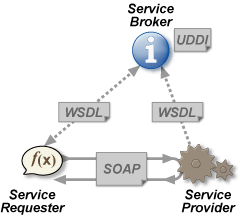
\includegraphics[width=4cm]{web-services}
    \end{figure}
  \end{columns}
\end{onlyenv}
\end{frame}

\begin{frame}[fragile,t]
\frametitle{Web 服务示例}

\begin{itemize}
\item http://www.webservicex.net/globalweather.asmx
\item \only<1| handout:1>{通过 SOAP 的访问} \only<2| handout:0>{返回的结果}
\end{itemize}

\begin{onlyenv}<1| handout:1>
\begin{lstlisting}[language=XML, showstringspaces=false]
POST /globalweather.asmx HTTP/1.1
Host: www.webservicex.net
Content-Type: text/xml; charset=utf-8
Content-Length: length
SOAPAction: "http://www.webserviceX.NET/GetWeather"

<?xml version="1.0" encoding="utf-8"?>
<soap:Envelope xmlns:xsi= ... >
 <soap:Body>
  <GetWeather xmlns="http://www.webserviceX.NET">
   <CityName>Harbin</CityName>
   <CountryName>China</CountryName>
  </GetWeather>
 </soap:Body>
</soap:Envelope>
\end{lstlisting}
\end{onlyenv}

\begin{onlyenv}<2| handout:0>
\begin{lstlisting}[language=XML, showstringspaces=false]
HTTP/1.1 200 OK
Content-Type: text/xml; charset=utf-8
Content-Length: length

<?xml version="1.0" encoding="utf-8"?>
<soap:Envelope xmlns:xsi= ... >
 <soap:Body>
  <GetWeatherResponse
           xmlns="http://www.webserviceX.NET">
   <GetWeatherResult>string</GetWeatherResult>
  </GetWeatherResponse>
 </soap:Body>
</soap:Envelope>
\end{lstlisting}
\end{onlyenv}
\end{frame}

\begin{frame}
\frametitle{公共语言基础结构}
\framesubtitle{实现 .NET 平台的基础}
\begin{block}{\textit{Common Language Infrastructure(CLI)}}
  \CJKindent CLI 定义了一个与平台无关的虚拟代码执行环境。包括公共中间语言和公
  共类型系统,相应的语法、语义和部分 .NET 框架类库。
\end{block}
\begin{itemize}
\item<2-| handout:1> CLI 中没有指定操作系统,可以在任何的系统或设备上实现
\item<3-| handout:1> 其他公司也可以根据 CLI 标准实现相关技术
  \begin{itemize}
  \item Microsoft .NET Framework --- 微软公司自己的实现
  \item Shared Source CLI --- 微软的开源 CLI
  \end{itemize}
\item<4-| handout:1> 目前已有的开源 .NET 平台
  \begin{itemize}
  \item Mono Project --- http://www.mono-project.com
  \item DotGNU Project --- http://www.dotgnu.org
  \end{itemize}
\end{itemize}
\end{frame}


\begin{frame}
\frametitle{公共语言基础结构}
\begin{figure}
\centering 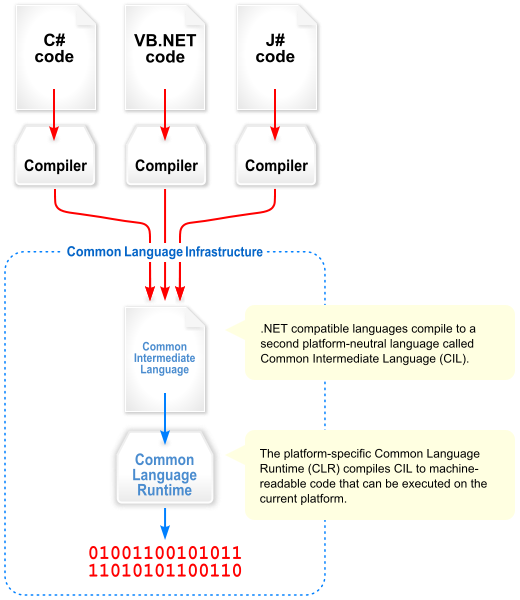
\includegraphics[height=7.5cm]{otl-cli}
\end{figure}
\end{frame}

\begin{frame}
\frametitle{CLI 的内容}

\begin{itemize}
\CJKindent
\item 概念和体系结构

  描述了 CLI 的体系结构,公共类型系统 (CTS)、虚拟执行系统 (VES)和公共语言规范 (CLS)的标准。

\item 元数据的定义和语法

  元数据的标准化定义:文件中的物理布局、逻辑内容,以及针对编译器的语法结构。

\item 公共中间语言(CIL)的指令集

  类似汇编语言的指令集,指令的语法结构。

\item 相关文件和库
\item 针对调试的中间格式

\end{itemize}

\end{frame}

\section{.NET 框架简介}

\begin{frame}
\frametitle{Microsoft .NET Framework}
\framesubtitle{功能丰富的开发平台}

\centering 
\includegraphics[width=4cm]{logo-dn}

\CJKindent 对开发人员来说 .NET 一般就是 .NET Framework,.NET Framework SDK 和 Visual Studio .NET
三个方面。

\begin{itemize}
\item \large 基于互联网的分布式应用程序
\item \large 创建与运行 Windows 应用程序的基础
\item \large 创建与使用 Web Services 的工具
\item \large 便携设备的开发和运行的环境
\end{itemize}
\end{frame}

\begin{frame}[t]\frametitle{Microsoft .NET Framework}
\framesubtitle{功能丰富的开发平台}
\begin{exampleblock}{提供了丰富的类库}
  \begin{columns}
    \column{4cm}
    \begin{itemize}
    \item ASP.NET
    \item Windows Forms
    \item Enterprise Services
    \end{itemize}
    \column{4cm}
    \begin{itemize}
    \item ADO.NET
    \item Web Services
    \item ...
    \end{itemize}
  \end{columns}
\end{exampleblock}
\begin{onlyenv}<2| handout:0>
  \begin{itemize}
  \item 充分利用代码复用,简化了应用程序的开发
  \item 类库提供开发所需的各种基本功能,可以支持各种类型的应用程序
  \item 类库屏蔽了底层细节,统一了编程模式,易于使用
  \item 容易维护、部署等
  \end{itemize}
\end{onlyenv}
\begin{onlyenv}<3| handout:1>
  \begin{block}{完整的安全解决方案}
    \begin{itemize}
    \item 基于证据的安全规则,确保组件的来源可靠
    \item 细致的权限设置,可以为组件设置不同权限
      \begin{itemize}
      \item 访问注册表
      \item 文件读取
      \item 访问网络
      \end{itemize}
    \end{itemize}
  \end{block}
\end{onlyenv}
\end{frame}

\begin{frame}
\frametitle{.NET 框架的组成}
\begin{itemize}
\item 公共语言运行时 --- \textit{Common Language Runtime}
\item .NET 框架类库 --- \textit{Framework Class Library}
\end{itemize}

\only<1| handout:1>{\label{fig:dn-framework}}
\centering %% Slides for ".NET Programming" by Chunyu Wang <chunyu@hit.edu.cn> %% -*- coding: utf-8 -*-

\begin{tikzpicture}[rounded corners,font=\small]

\draw[fill=yellow!10,opacity=.5] (  0,  0) rectangle +(11, 5.5);
\filldraw[black!20!white] (.8,.2) rectangle +(9.4, .6); 
\node at (5.5, .5) {操作系统或移动设备};

\draw[dashed] (.6,1) rectangle +(9.8, 3.2);

\visible<2-| handout:1>{\filldraw[red!20] (.8,1.2) rectangle +(9.4, .6); 
\node at (5.5, 1.5) {公共语言运行时 ~CLR};}

\visible<3-| handout:1>{\filldraw[blue!20] (.8,  2) rectangle +(9.4,  2); 
\node at (5.5, 2.3) {.NET 框架类库 ~FCL};
\tikzstyle{fltext}=[fill=blue!30,anchor=west,rectangle,font=\color{black}\footnotesize]
\draw (.9, 3.2) node[text centered, text width=0.9cm, style=fltext] {ASP .NET}; 
\draw (2.2,3.2) node[text centered, text width=1.6cm, style=fltext] {Windows Forms};                         
\draw (4.2,3.2) node[text centered, text width=1.6cm, style=fltext] {Web Service};
\draw (6.2,3.2) node[text centered, text width=1.8cm, style=fltext] {Enterprise Service};
\draw (8.4,3.2) node[text centered, text width=0.9cm, style=fltext] {ADO .NET};
\draw (9.5,3.2) node[anchor=west,ultra thick] {$\dots$};}

\draw[fill=yellow!70!cyan!60!white,draw=gray,font=\color{black}] (6.0, 4.8) ellipse (1.5cm and .5cm);
\draw[fill=yellow!70!cyan!60!white,draw=gray,font=\color{black}] (5.5, 4.8) ellipse (1.5cm and .5cm);
\draw[fill=yellow!70!cyan!60!white,draw=gray,font=\color{black}] (5.0, 4.8) ellipse (1.5cm and .5cm);
\node at (5.0,4.8) {应用程序};

\end{tikzpicture}

\end{frame}

% \begin{frame}
% \frametitle{代码重用和DLL}
% \setlength{\itemsep}{6pt plus 1pt}
% \begin{itemize}
% \item 代码重用,提高效率,减少二次开发 \pause
% \item 动态加载需要组件,减少内存使用 \pause
% \item 维护 DLL 需要特别的认真仔细
%   \begin{itemize}
%   \item 版本唯一,向下兼容,保证代码正确执行
%   \item 仔细实现错误检查,无法处理的错误要通过固定的错误码向上提交
%   \item 处理与其他 DLL 之前的联系,保持兼容
%   \end{itemize}
% \pause
% \item 当旧版本的 DLL 覆盖新的 DLL 时,会发生 DLL Hell
% \item 解决 DLL Hell --- .NET 的设计动机之一
% \end{itemize}
% \end{frame}

\begin{frame}[t]
\frametitle{.NET 框架的各个版本}

\begin{columns}[t]
\column{.58\textwidth}
\begin{itemize}[<+->]
\small
\item Framework 1.0 (2002-2-13)

\only<.| handout:0>{ \CJKindent 初次发布,支持 Win 98, NT 4.0, 2000, XP。}

\item Framework 1.1 (2003-4-3)

\only<.| handout:0>{
\begin{itemize}
\item<.-> ASP.NET, ADO.NET
\item<.-> .NET Compact Framework
\item<.-> 包含在 Visual Studio 2003 中
\end{itemize}}

\item Framework 2.0 (2005-11-7)

\only<.| handout:0>{
\begin{itemize}
\item<.-> 语言的改进,如支持范型等
\item<.-> 控件的增加和改进
\item<.-> 免费的SDK 下载
\item<.-> 随Visual Studio 2005, Microsoft SQL Server 2005 一起发布
\end{itemize}}

\item Framework 3.0 (2006-11-21)

\only<.| handout:0>{
\begin{itemize}
\item<.-> 仍然使用 2.0 的框架,但增加了新成员 WPF, WCF, WF 和 CardSpace
\item<.-> 是 Windows Vista 和 Windows Server 2008 的一部分
\end{itemize}}

\item Framework 3.5 (2007-11-19)

\only<.| handout:0>{
\begin{itemize}
\item<.-> 语言的改进,C\# 3.0 和VB.NET 9.0
\item<.-> LINQ(Language Integrated Query)
\item<.-> ASP.NET AJAX
\end{itemize}}

\item Framework 4.0 (2010-04-12)

\only<.| handout:0>{
\begin{itemize}
\item<.-> DLR, 并行扩展,PLINQ
\item<.-> IronPython, IronRuby, F\# 的完整支持
\item<.-> Visual Studio 2010
\end{itemize}}

\item Framework 4.5 (2012-8-15)

\only<.| handout:0>{
\begin{itemize}
\item<.-> HTML5, Metro界面(Win8)
\item<.-> Windows Phone \ldots
\end{itemize}}
\end{itemize}

\column{.41\textwidth}
\begin{figure}
\centerline{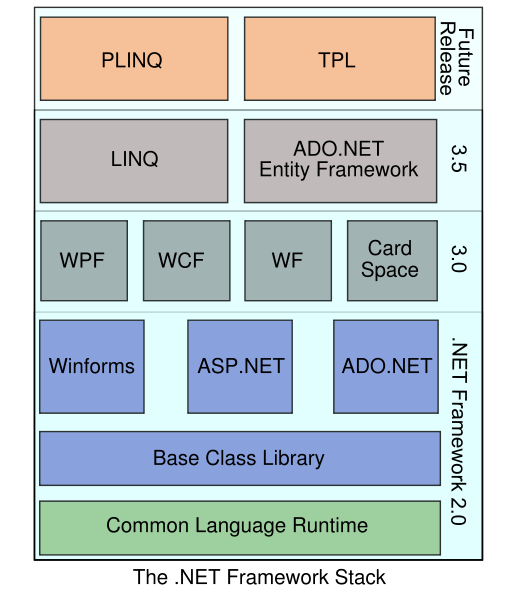
\includegraphics[width=4cm]{otl-dotnet}}
\end{figure}
\end{columns}
\end{frame}


\section{公共语言运行时}

\begin{frame}
\frametitle{公共语言运行时}
\begin{block}{\textit{Common Language Runtime(CLR)}}
  \CJKindent 全部 .NET Framework 的基础,为 .NET 程序提供了一个虚拟机环境,
  以支持进程的创建和执行,托管代码和非托管代码的交互,为进程提供必要的服务。
\end{block}

% \begin{figure}[h] \only<1-| handout:1>{\label{fig:clr-compile-exec}}
%   \centering \begin{tikzpicture}[rounded corners, >=stealth]
\tikzstyle{tnode}=[fill=red!30, text width=1.7cm, rounded corners,
minimum height=1.1cm, minimum width=1.7cm, anchor=south west, font=\footnotesize]
\draw[dashed,fill=blue!20, fill opacity=.4] (.7, .5) rectangle +(8.4,1.8);
\draw[dashed,fill=blue!20, fill opacity=.4] (.7,2.5) rectangle +(8.4,1.9);

\draw (1,2.7) node[style=tnode] (aa) {����Դ��} ;   
\draw (4,2.7) node[style=tnode] (bb) {������} ; 
\draw (7,2.7) node[style=tnode] (cc) {�����} ;
\draw (4,1)   node[style=tnode] (dd) {JIT������} ;  
\draw (1,1)   node[style=tnode] (ee) {���ش���} ;   

\draw (4.5,.8)  node {����ִ��};
\draw (4.5,4.1) node {�������};

\draw[->] (aa.east) -- (bb.west);
\draw[->] (bb.east) -- (cc.west);
\draw[->] (dd.west)--(ee.east);
\draw[->] (cc.south) .. controls (cc.south|-dd.east) .. (dd.east);
\end{tikzpicture}

% \end{figure}

\begin{itemize}
\item<2-| handout:1> CLR 要管理\alert<2| handout:0>{托管代码}的整个运行周期:查找代码、编译、加载相
  关的类、运行、自动内存管理
\item<3-| handout:1> 提供多种语言都支持的\alert<3| handout:0>{公共类型系统},定义如何声
  明和管理 CLR 中的类型
\item<4-| handout:1> 支持跨语言集成,允许不同语言之间的交互
\item<4-| handout:1> 管理类型系统的安全,管理组件的安全
\item<4-| handout:1> 访问其他系统资源,提供 Win32 API, COM 等访问接口
\end{itemize}

% \begin{itemize}
% \item 提供通用类型系统 (CTS)\\
%   值类型:整数、浮点数、结构体等\\
%   引用类型:类对象、委托、接口等
% \item 为托管代码执行提供服务\\
%   智能内存管理,元数据管理,受管库的加载与分析,处理异常,代码互操作
% \item 访问系统资源\\
%   Win32 API 或 COM 等
% \end{itemize}
\end{frame}

\begin{frame}
\frametitle{托管代码}

\begin{block}{\textit{Managed Code}}
  \CJKindent 托管代码是由面向 CLR 的编译器生成,支持公共语言运行时服务的代码,为了支持这些服务,代码必须向运行时提供最小级
  别的信息,即元数据 (\textit{metadata})。
\end{block}

\pause
\begin{itemize}
\item 托管代码的运行受 CLR 控制,如内存分配、类型检查、安全验证、垃圾回收等
\item 由公共语言运行时的垃圾回收器进行分配和释放的数据,称为托管数据
\item 默认情况下,所有 C\#, Visual Basic.NET 和 JScript.NET 代码都是托管代码
\item Visual Studio.NET C++ 默认情况下不是,但通过编译器命令行开关 (\texttt{/CLR}),也可以生成托管代码
\end{itemize}
\end{frame}

\begin{frame}
\frametitle{CLR 虚拟机}
\begin{itemize}
\item<1-| handout:1> CLR 相当于一种虚拟机,独立于操作系统或体系结构
\item<2-| handout:1> .NET 编译器生成 Windows PE (\textit{Portable Executable}) 文件,扩展名通常
  为 DLL 或 EXE
\item<3-| handout:1> Windows PE 文件实际内容是面向 CLR 的中间语言文件,以及执行所需的 CLR 文件头
\item<4-| handout:1> 当执行时,通过调用 JIT (\textit{Just-In-Time}) 编译器,实时编译为本地代码
  (\textit{native code})
\end{itemize}

\begin{figure}[h] \only<1| handout:1>{\label{fig:clr-compile-exec}}
  \centering \begin{tikzpicture}[rounded corners, >=stealth]
\tikzstyle{tnode}=[fill=red!30, text width=1.7cm, rounded corners,
minimum height=1.1cm, minimum width=1.7cm, anchor=south west, font=\footnotesize]
\draw[dashed,fill=blue!20, fill opacity=.4] (.7, .5) rectangle +(8.4,1.8);
\draw[dashed,fill=blue!20, fill opacity=.4] (.7,2.5) rectangle +(8.4,1.9);

\draw (1,2.7) node[style=tnode] (aa) {����Դ��} ;   
\draw (4,2.7) node[style=tnode] (bb) {������} ; 
\draw (7,2.7) node[style=tnode] (cc) {�����} ;
\draw (4,1)   node[style=tnode] (dd) {JIT������} ;  
\draw (1,1)   node[style=tnode] (ee) {���ش���} ;   

\draw (4.5,.8)  node {����ִ��};
\draw (4.5,4.1) node {�������};

\draw[->] (aa.east) -- (bb.west);
\draw[->] (bb.east) -- (cc.west);
\draw[->] (dd.west)--(ee.east);
\draw[->] (cc.south) .. controls (cc.south|-dd.east) .. (dd.east);
\end{tikzpicture}

\end{figure}
\end{frame}


\begin{frame}
\frametitle{公共类型系统}

\begin{block}{\textit{Common Type System(CTS)}}
  \CJKindent CTS 是一组预定义的类型和这些类型行为的规范,描述了如何声明和创建
  定制类型,如何管理这些类型实例的生命周期,以及怎样才能得到 CLR 的支持。
\end{block}

\begin{uncoverenv}<2-| handout:1>
  \begin{itemize}
  \item 定义了声明、使用和管理定制或预定义类型的标准化框架
  \item 使不同的编程语言之间的能够集成
  \item 遵循 CTS 能够保障类型的安全和性能的优化
  \item 遵循 CTS 的语言不一定支持 CTS 中定义的全部类型
  \end{itemize}
\end{uncoverenv}
\end{frame}

\begin{frame}[c]
\frametitle{CTS 的类型结构}

% 所有的类型都派生自Objects类型,而所有的值类型都派生自ValueTypes类型。
\begin{figure}[h]  \only<1| handout:1>{\label{fig:cts-typesystem}}
  \centering  %% Slides for ".NET Programming" by Chunyu Wang <chunyu@hit.edu.cn> %% -*- coding: utf-8 -*-

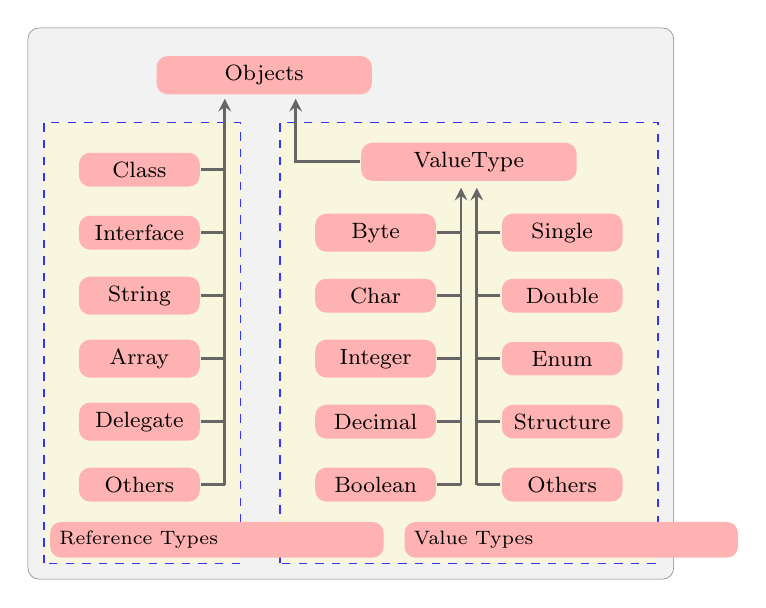
\begin{tikzpicture}[line width=1pt, >=stealth, draw=black!60]
\tikzstyle{every_node}=[font=\color{black}\footnotesize, text width=1.3cm, text centered, fill=red!30, rounded corners]
\tikzstyle{nnnn}=[anchor=center, text width=4cm, font=\color{black}\scriptsize]
\filldraw[fill=gray!10, draw=gray, line width=.2pt, rounded corners] (-.2,.8)  rectangle +(8.2, 7);

\filldraw[anchor=center] (2.8,7.2) node[style=every_node,text width=2.5cm] {Objects};

\filldraw[fill=yellow!20, fill opacity=.5, line width=.6pt,draw=blue!80, dashed] (0,1) rectangle +(2.5,5.6);
\filldraw[fill=yellow!20, fill opacity=.5, line width=.6pt,draw=blue!80, dashed] (3,1) rectangle +(4.8,5.6);
\filldraw (2.2, 1.3) node[style=nnnn] {Reference Types};
\filldraw (6.7, 1.3) node[style=nnnn] {Value Types};

\filldraw[anchor=center] (5.4,6.1) node[style=every_node,text width=2.5cm] (vt) {ValueType};
\draw[->] (vt) -| (3.2,6.9);

\foreach \a/\b in {2/Others,2.8/Delegate,3.6/Array,4.4/String,5.2/Interface,6/Class}
{\filldraw (2, \a ) node[style=every_node,anchor=east] {\b};
  \draw (2, \a ) -- (2.3, \a );}
\draw[->] (2.3,2) -- (2.3,6.9);
\foreach \a/\b in {2/Boolean,2.8/Decimal,3.6/Integer,4.4/Char,5.2/Byte}
{\filldraw (5, \a ) node[style=every_node,anchor=east] {\b};
  \draw (5, \a ) -- (5.3, \a );}
\draw[->] (5.3,2) -- (5.3,5.77);
\foreach \a/\b in {2/Others,2.8/Structure,3.6/Enum,4.4/Double,5.2/Single}
{\filldraw (5.8, \a ) node[style=every_node,anchor=west] {\b};
  \draw (5.8, \a ) -- (5.5, \a );}
\draw[->] (5.5,2) -- (5.5,5.77);
\end{tikzpicture}

\end{figure}
\end{frame}


\begin{frame}
\frametitle{值类型和引用类型}
% 值类型和引用类型的区别:
% http://msdn2.microsoft.com/en-us/library/2hf02550.aspx
\begin{itemize}
\item<1-| handout:1> \small CLR 是一种基于栈的虚拟机,并维护一个用于创建对象的堆
\item<2-| handout:1> \small 函数调用时自动分配的内存在栈中,当函数返回时自动释放
\item<3-| handout:1> \small 自由创建的对象在堆中,栈中只有堆中地址的引用 (\textit{reference}) \\
  \small 堆中分配的对象不会自动释放,而是由垃圾回收负责
\item<4-| handout:1> \small 在栈中分配的变量是值类型的,而堆中的是引用类型
\end{itemize}

\begin{columns}
  \column{.5\textwidth}
  \begin{figure}[h] \only<1| handout:1>{\label{fig:cts-v-r-types}}
    \centering %% Slides for ".NET Programming" by Chunyu Wang <chunyu@hit.edu.cn>

\begin{tikzpicture}[>=stealth]
\fill[fill=yellow!10,draw=gray,fill opacity=.5, rounded corners] (.5 ,0) rectangle +(7.5,5.5) ;

\node[anchor=center] at (2, 0.5) {�й�ջ};

\filldraw[draw=black,fill=blue!20,fill opacity=.4,rounded corners] (1,1) rectangle +(2,4);
\filldraw[draw=black,fill=red!40] (1,2) rectangle +(2,1);
\draw (1,4) -- (3,4);
% \draw (1,3) -- (3,3);
% \draw (1,2) -- (3,2);
\filldraw[draw=black,fill=blue!20,fill opacity=.4,dashed,rounded corners] (4,1) rectangle +(3.5,3.5);
\fill[red!40,rounded corners] (4.75, 2) rectangle +(2,1);
\foreach \a/\b in {1.5/����: 43, 2.5/�ַ���:, 3.5/�ַ���: A, 4.5/����:124}
\node[anchor=west, font=\small] at (1, \a ) {\b};

\node[anchor=center] at (5.75, 0.5) {�йܶ�};
\draw (5.75, 2.5) node[anchor=center] (a) {Hello};

\draw[->,thick] (2.75,2.5) .. controls (3.45,2.8) and (4.15,2.8) .. (a.west);

\end{tikzpicture}

  \end{figure}
  \column{.5\textwidth}
  \begin{itemize}
  \item<1-| handout:1> \small 托管栈 --- \textit{Managed Stack}
  \item<1-| handout:1> \small 托管堆 --- \textit{Managed Heap}
  \item<4-| handout:1> \small 值类型 --- \textit{Value Type}
  \item<4-| handout:1> \small 引用类型 --- \textit{Reference Type}
  \end{itemize}

\end{columns}
% 托管代码执行过程中,变量可以在托管栈或托管堆中分配。
% 当方法被调用时,局部变量或方法创建的值类型变量都在栈中分配,当方法运行结束时都自动的释放;
% 而在堆中分配的变量,并不自动释放,而是通过“垃圾处理”来由CLR管理并释放。

% 值类型的变量在栈中分配,而引用类型的变量在栈中只有一个引用,指向在堆中实际内存

\end{frame}

\begin{frame}
\frametitle{公共语言规范}
\begin{block}{\textit{Common Language Specification(CLS)}}
  \CJKindent 语言互操作的最终规范,定义了遵循 CLR 的编译器必须包含的最小特性集,保证语
  言之间的通信。% CTS 的一个子集。
\end{block}

\begin{exampleblock}{部分 CLS 特性和规则}<2-| handout:1>
  % \rowcolors{1}{RoyalBlue!20}{RoyalBlue!5}
  \begin{tabular}{l|l}
    \hline \multicolumn{1}{c|}
    {\bfseries 特\ \ 性} & \multicolumn{1}{c}{\bfseries 规\ \ 则}          \\\hline
    可见性         & 定义类型的程序集之外有效                   \\
    字符和大小写   & 变量除了大小写不同之外,还需要有其他区别   \\
    基本类型       & Byte, Int, Single, Double, Boolean 等      \\
    构造函数调用   & 访问实例数据前,必须调用基类的构造函数     \\
    数组边界       & 数组的各个维下界必须为 0                  \\
    枚举           & 基类型必须是 Byte, Int16, Int32 或 Int64 \\
    方法签名       & 签名中返回值和参数的类型必须遵循 CLS      \\
  \end{tabular}
\end{exampleblock}

\end{frame}



% \subsection*{托管代码的编译}
\begin{frame}<0| handout:0>
\frametitle{CLR 中程序的运行}
\begin{itemize}
\item CLR 定义了一种基于栈的虚拟机
\item CLR 上执行的代码是 CIL 编写的托管代码
\item CIL 通过 JIT 实时的编译为本地代码
\item CLR 是负责托管代码执行的虚拟运行环境
\item MSIL 是 CIL 的一种实现
\end{itemize}
\end{frame}

\begin{frame}
\frametitle{Microsoft 中间语言}
% 什么是 Microsoft 中间语言 (MSIL)?

\begin{block}{\textit{Microsoft Intermediate Language}}
  \CJKindent MSIL 是与 CPU 无关的指令集,它包含加载、存储、初始化和调用对象方法
  的指令,相当于 CLR 的汇编语言。
\end{block}
\pause

\begin{itemize}
\item \small .NET 框架程序被编译成生成 MSIL 和元数据
\item \small MSIL,元数据,CTS 结合,允许真正的跨语言集成
\item \small MSIL 在执行前被转换为机器代码,而不是边解释边执行
\end{itemize}
\pause

\begin{figure}[h] \only<1| handout:1>{\label{fig:clr-compile}}
  \centering 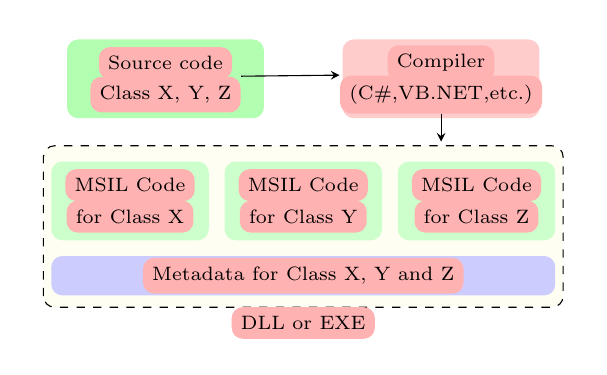
\begin{tikzpicture}[font=\scriptsize, rounded corners, >=stealth]
\path[fill=white,fill opacity=.4] (1.5,.85) rectangle (8.5,4.9);
\path[fill=green!30] (2,3.75) rectangle +(2.5,1) 
+(1.25,.3) node (a) {Class X, Y, Z} +(1.25,.7) node {Source code};
\path[fill=red!20] (5.5,3.75) rectangle +(2.5,1) 
+(1.25,.3) node (b) {(C\#,VB.NET,etc.)} +(1.25,.7) node {Compiler};
\draw[->] (a.north east) -- (b.north west);
\draw[->] (b.south) -- +(down:.35cm);
\draw[dashed,fill=yellow!5] (1.7,1.35) rectangle (8.3,3.4) (5,1.15) node {DLL or EXE};
\foreach \x/\y in {-2.2cm/X,0cm/Y,2.2cm/Z} 
\path[fill=green!20,xshift=\x] (4,2.2) rectangle +(2,1) +(1,.7) node {MSIL Code} +(1,.3) node {for Class \y} ;
\path[fill=blue!20] (1.8,1.5) rectangle +(6.4,.5) +(3.2,.25) node {Metadata for Class X, Y and Z};
\end{tikzpicture}

\end{figure}

\end{frame}

\begin{frame}
\frametitle{ .NET PE 文件}
\begin{block}{\textit{.NET Portable Executable File}}
\CJKindent \small  为支持 CLR 扩展的 Windows PE 文件格式。其中包括了 PE 文件的头信息,CLR 的头信息,程序的元数据和
  IL 代码以及数据段。
\end{block}
\pause
\begin{columns}
  \column{.4\textwidth}
  \begin{figure}[htbp]
    \centering
    %% Slides for ".NET Programming" by Chunyu Wang <chunyu@hit.edu.cn>

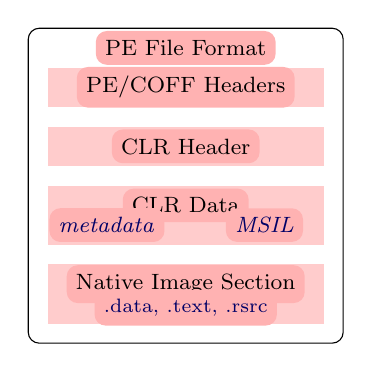
\begin{tikzpicture}[font=\footnotesize]
\draw[rounded corners] (0,.25) rectangle (4,4.25);
\fill[red!20] (.25,.5) rectangle +(3.5,.75);
\fill[red!20] (.25,1.5) rectangle +(3.5,.75);
\fill[red!20] (.25,2.5) rectangle +(3.5,.5);
\fill[red!20] (.25,3.25) rectangle +(3.5,.5);
\node at (2,4) {PE File Format};
\node at (2,3.5) {PE/COFF Headers};
\node at (2,2.75) {CLR Header};
\node at (2,2) {CLR Data};
\node at (1,1.75) {\color{blue!40!black}\textit{metadata}};
\node at (3,1.75) {\color{blue!40!black}\textit{MSIL}};
\node at (2,1) {Native Image Section};
\node at (2,.7) {\color{blue!40!black}\scriptsize .data, .text, .rsrc};
\end{tikzpicture}

  \end{figure}
  \column{.6\textwidth}
\pause
\begin{itemize}
\item 查看 PE 文件内容\\
{\footnotesize \cmd{dumpbin.exe Hello.exe}}
\vskip4pt
\item \textit{Core execution engine} \\
{\color{red!40!black} \texttt{mscoree.dll}\\
\texttt{...}\\
\texttt{$\_$CorExeMain}}

\end{itemize}
\end{columns}

\end{frame}

\begin{frame}
\frametitle{托管代码的实时编译}
\begin{overlayarea}{\textwidth}{1.2cm}
  \begin{itemize}
  \item \small
    \only<1| handout:0> {当托管代码调用其他模块或方法时, CLR 自动寻找并将其加载}
    \only<2| handout:0> {然后跳转到该方法的入口,首先调用 \texttt{\_CorExeMain()} 方法,通过它检查当前代
      码是否已经被编译为本地代码}
    \only<3| handout:0> {如果没有编译,则调用 JIT 编译器,把当前方法的 MSIL 编译为本地代码}
    \only<4| handout:0> {并将原来加载 MSIL 代码替换为本地代码}
    \only<5| handout:0> {因为已经替换了内存中的内容,所以 MSIL 加载之后,只需编译一次 }
    \only<6| handout:0> {当方法再次被调用时,可以直接执行,不需再次编译}
    \only<0| handout:1> {已经编译的本地代码会替换内存中的 MSIL,因此无需再次编译}
  \end{itemize}
\end{overlayarea}

\begin{figure}[h] \only<1| handout:1>{\label{fig:clr-execute}}
  \centering %% Slides for ".NET Programming" by Chunyu Wang <chunyu@hit.edu.cn>
%% $LastChangedDate$
%% $Rev$

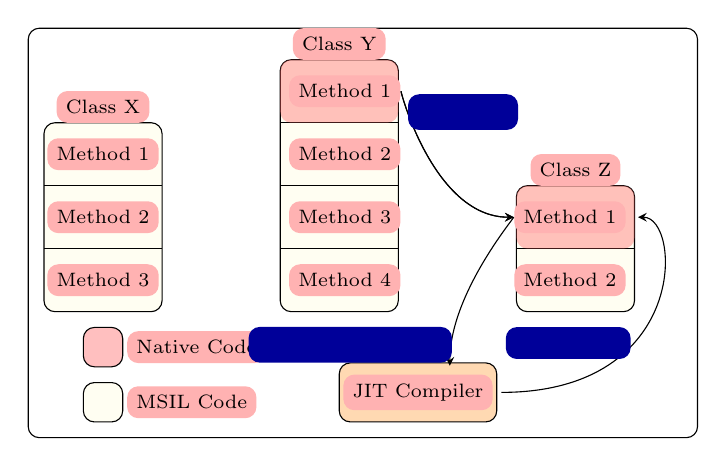
\begin{tikzpicture}[font=\scriptsize, rounded corners, >=stealth]
\def\rowstroke{++(0cm,.8cm) -- +(1.5,0)}
\draw[fill=white,fill opacity=.4] (-.2,.4) rectangle (8.3,5.6);

\path[draw,fill=yellow!5] (0,2) rectangle +(1.5cm,.8cm*3);
\draw (0,2) \rowstroke \rowstroke;
\foreach \x in {1,2,3}\draw (0,2) +(.75cm,2.8cm-.8cm*\x) node {Method \x};
\draw (.75,4.6) node {Class X};

\path[draw,fill=yellow!5] (3,2) rectangle +(1.5cm,.8cm*4);
\draw (3,2) \rowstroke \rowstroke \rowstroke;
\fill[color=red!60,fill opacity=.4] (3cm,4.4cm) rectangle +(1.5cm,.8cm) ;
\foreach \x/\y in {1/y1,2/y2,3/y3,4/y4} \draw (3,2) +(.82cm,3.6cm-.8cm*\x) node (\y) {Method \x};
\draw (3.75,5.4) node {Class Y};

\path[draw,fill=yellow!5] (6,2) rectangle +(1.5cm,.8cm*2);
\draw (6,2) \rowstroke;
\fill<4->[color=red!60,fill opacity=.4] (6cm,2.8cm) rectangle +(1.5cm,.8cm) ;
\foreach \x/\y in {1/z1,2/z2} \draw (6,2) +(.68cm,2cm-.8cm*\x) node (\y)  {Method \x};
\draw (6.75,3.8) node {Class Z};

\fill[draw,fill=yellow!5] (.5, .6) rectangle +(.5,.5) +(.55,.25) node[anchor=west] {MSIL Code};
\fill[draw,fill=red!25,pos=.35]   (.5,1.3) rectangle +(.5,.5) +(.55,.25) node[anchor=west] {Native Code};

\path[xshift=1cm,draw,fill=orange!30] (2.75,.6) rectangle +(2,.75) +(1,.375) node (jit) {JIT Compiler};

\draw<2| handout:1>[->] (y1.east) .. controls +(down:1pt) and +(left:1cm) 
.. node[blue!60!black,near start,right] {\sl First Call} (z1.west);
\draw<3| handout:1>[->,shorten >=3pt] (z1.west) .. controls +(250:1pt) and +(up:1cm) 
.. node[blue!60!black,very near end,left] {\sl Compile MSIL Code} (jit.30);
\draw<4| handout:1>[->,shorten >=.15cm, shorten <=3pt] (jit.east) .. controls +(right:2.5cm) and +(right:.7cm)
.. node[blue!60!black,pos=.35,left] {\sl Native code} (z1.east);
\draw<6| handout:0>[->] (y1.east) .. controls +(down:1pt) and +(left:1cm)
.. node[blue!60!black,near start,right] {\sl Call again} (z1.west);
\end{tikzpicture}

\end{figure}

\end{frame}

\begin{frame}
\frametitle{生成本地镜像}
\begin{block}{\textit{Native Image Generator}}
  \CJKindent \small SDK 提供的用于产生本地代码镜像工具 ngen.exe,可以将文件一次性转换为本地代码。
\end{block}
\vskip4pt
\cmd{csc /t:exe /out:Hello.exe Hello.cs}
\cmd{ngen Hello.exe}
\cmd{Hello.exe}
\vskip4pt
\begin{itemize}
\item 可以提高执行效率,防止过多使用 JIT 编译器
\item 产生的本地代码仍然需要 CLR 才能运行
\end{itemize}

\end{frame}

\begin{frame}
\frametitle{程序集}
\begin{block}{\textit{Assembly}}
  \CJKindent \small .NET 框架应用程序中,由一个或一组文件构成的,单一功能的
  逻辑单元。程序集是组件复用,实施安全策略的最小单位。
\end{block}
\pause
\begin{itemize}
\item 程序集可以有一个或多个文件
\item 程序集都有一个{\color<handout:0>{red!65!black}清单} (\textit{manifest}{})
\item 清单描述程序集的内容信息
  \begin{enumerate}
  \item 程序集的名字
  \item 版本号,形如 major.minor.build.revision
  \item 区域性信息(如支持的语言等)
  \item 程序集其他文件列表
  \item 所依赖的其他程序集及版本号
  \end{enumerate}
\end{itemize}
\end{frame}

\begin{frame}[t]
\frametitle{程序集的清单}

\begin{itemize}
\item 清单就是程序集的元数据,描述程序集包含的内容
\item 如 DLL 文件,EXE 文件,图片文件,数据文件等
\item 而程序集的清单只在其中一个文件中
\end{itemize}

  \begin{center}
    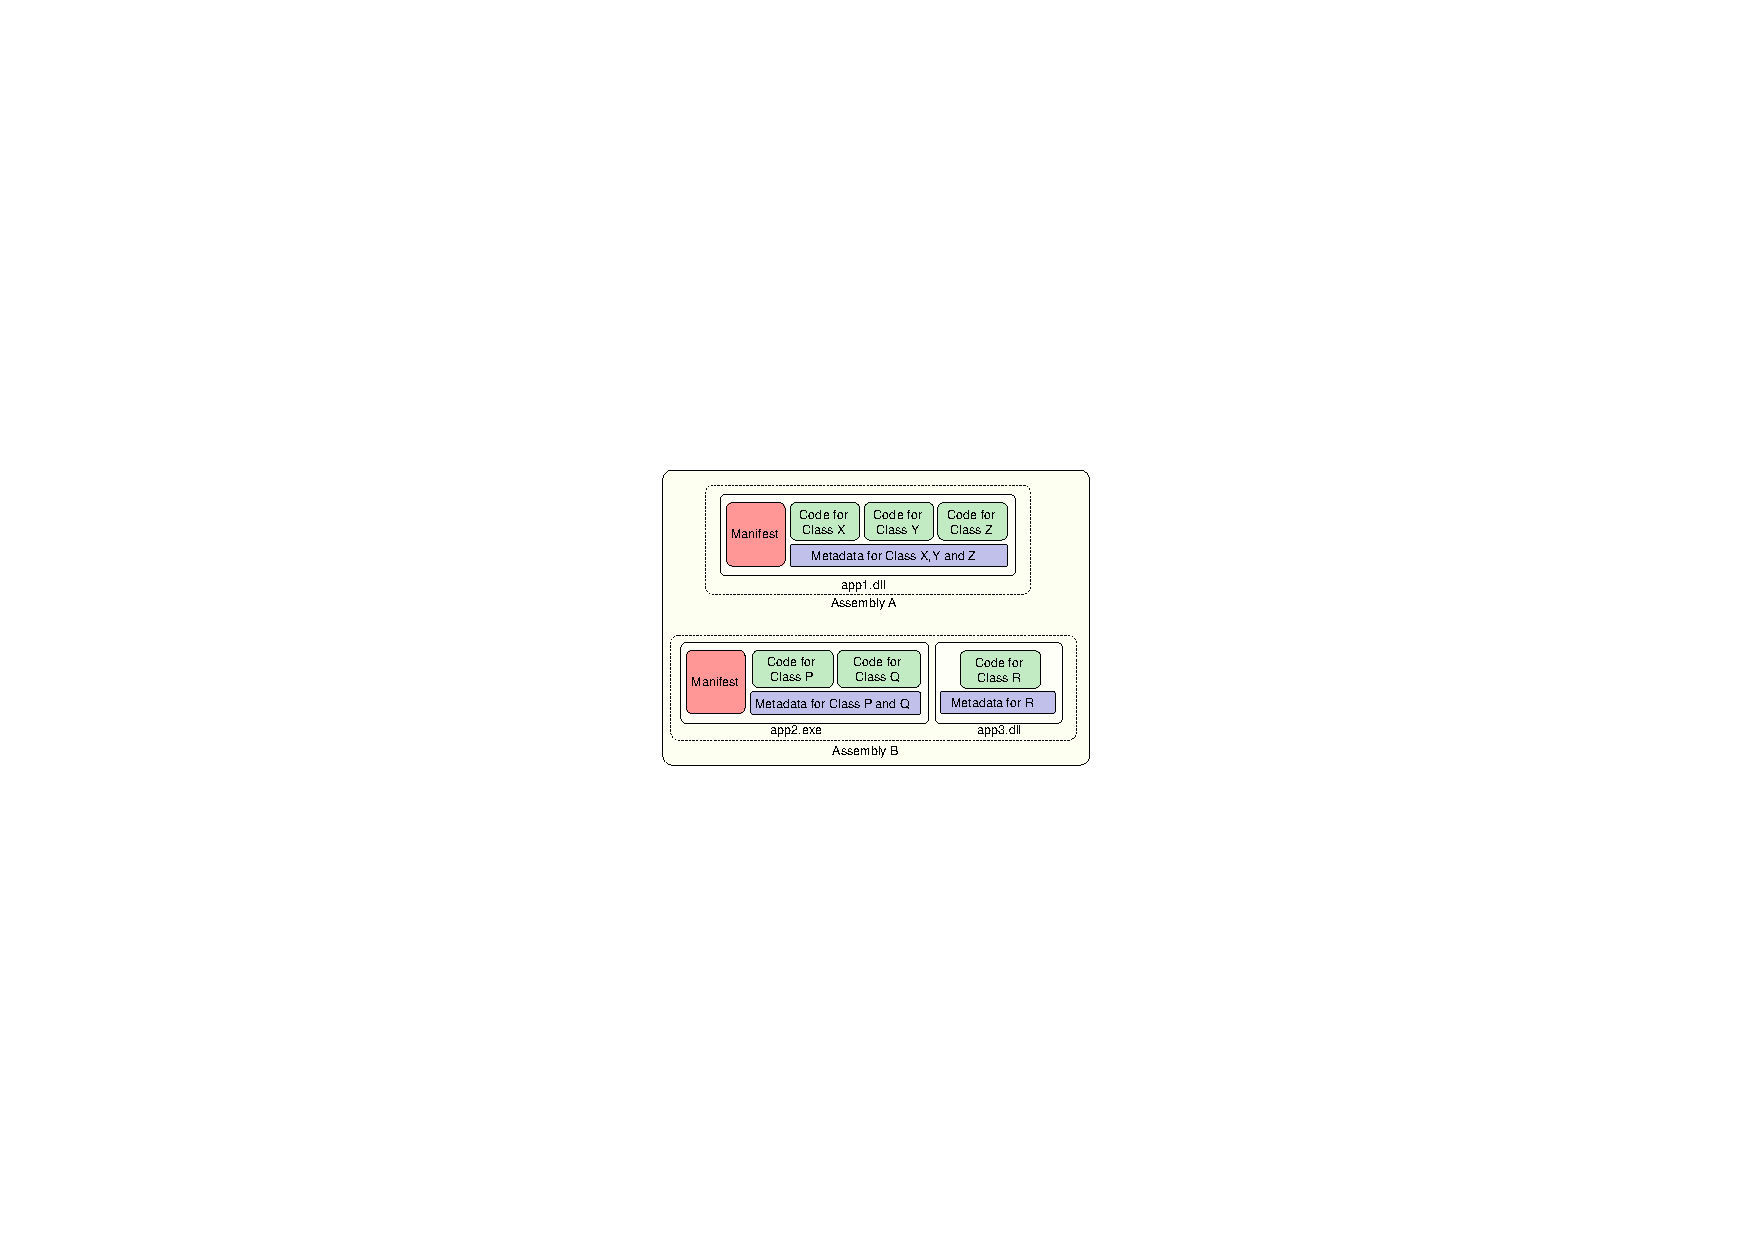
\includegraphics[angle=270]{assembly1.pdf}
  \end{center}
\end{frame}

\begin{frame}
\frametitle{程序集的功能}
\begin{itemize}
  \setlength{\itemsep}{10pt plus 1pt}
\item 程序集定义了类型的有效范围, CLR 通过程序集查找类
\item 程序集不需要注册表项, CLR 通过一种算法查找程序集
\item 安装 .NET 应用程序,只拷贝它的程序集即可\pause
  % 安装与卸载 .NET 模块不需要修改系统注册表,只需 copy or delete
\item 程序集可以有一个{\color<handout:0>{red!65!black}增强型名称} (\textit{Strong name}),用作共享名称
  \begin{itemize}
  \item 除了三个必须的成员(程序集名,版本号和区域性信息)之外,还要有数字签名和相应的公钥
  \item 通过数字签名,可以确保程序集的唯一性,增加安全性
  \end{itemize}

\item 允许不同版本的程序集并存,可有效避免 DLL Hell
  % 因为程序集需要指定版本号,而程序集的依赖也如此
\end{itemize}
\end{frame}

\begin{frame}
\frametitle{程序集的种类}
% http://www.microsoft.com/china/msdn/archives/library/faq111700.asp

\begin{block}{专用程序集}
  \CJKindent \small 专用程序集仅由单一应用程序使用,并且存储在该应用程序的安装目录中(或其子目录中)。要求在使
  用它的应用程序中是唯一的。
\end{block}
\pause
\begin{block}{共享程序集}
  \CJKindent \small 共享程序集是可被多个应用程序引用的程序集,通常被明确安装在全局程序集缓
  存 (\textit{Global Assembly Cache, GAC})中。要共享一个程序集,可以通过给其指定加密的增强型名称来实
  现。
\end{block}
\pause
\begin{itemize}
\item 通过区分专用和共享程序集,确定如何{\color<handout:0>{red!65!black}部署} (\textit{Deploy}) 程序集
\item 根据增强型名称,判断是否接受程序集,或新的版本
\item 根据版本管理特性,保证下载的代码不会影响本地应用程序的执行
\end{itemize}

\end{frame}

\begin{frame}
\frametitle{程序集的加载过程}
\begin{itemize}
  \setlength{\itemsep}{8pt plus 1pt}
\item 只有在需要的时候加载,程序集可以在本地或网络中

\item CLR 通过特定的规则寻找需要的程序集

  \begin{enumerate}
    \setlength{\itemsep}{4pt plus 1pt}
  \item CLR 检查是否已经被加载,如果已经加载,结束查找
  \item 在全局程序集缓存(GAC)中查找
  \item 在程序代码中指定的位置查找
  \item 如果代码没有指定,在应用程序目录查找
  \item 根据 .NET 的配置,在其他目录或 URL 查找
  \item 如果都未找到,报告错误,结束查找
  \end{enumerate}

\item 找到程序集后,检查增强名(如果有),加载并使用
\end{itemize}
\end{frame}


\begin{frame}
\frametitle{应用程序域}
\begin{block}{\textit{App Domain}}
  \CJKindent 应用程序域为安全性、可靠性、版本控制以及卸载程序集提供了隔离边界。应用程序域通常由运行库
  宿主创建,运行库宿主负责在运行应用程序之前引导公共语言运行库。
\end{block}
\pause
\begin{itemize}
\item 加载 CLR 的程序称为{\color<handout:0>{red!65!black}运行库宿主} (\textit{runtime host})
\item 应用程序域,由运行库宿主创建
\item 宿主依靠{\color<handout:0>{red!65!black}验证} (\textit{verification})来隔离程序集
\item 在一个应用程序域中出现的错误不会影响其他应用程序域
\end{itemize}
\end{frame}

% \begin{itemize}
% \item 在一个应用程序中出现的错误不会影响其他应用程序\par
%   \CJKindent \small 因为类型安全的代码不会导致内存错误,所以使用应用程序域可以确保在一个域中运行的代
%   码不会影响进程中的其他应用程序。
% \item 能够在不停止整个进程的情况下停止单个应用程序\par
%   \CJKindent \small 使用应用程序域使可以卸载在单个应用程序中运行的代码。不能卸载单个程序集或类型。只
%   能卸载整个域。
% \item 在一个应用程序中运行的代码不能直接访问其他应用程序中的代码或资源
% \item 代码行为的作用范围由它运行所在的应用程序决定\par
%   \CJKindent \small 换言之,应用程序域将提供应用程序版本策略等配置设置、它所访问的任意远程程序集的位
%   置,以及加载到该域中的程序集的位置信息。
% \item 向代码授予的权限可以由代码运行所在的应用程序域来控制
% \end{itemize}

\section{.NET 框架类库}

\begin{frame}
\frametitle{.NET 框架类库}

\begin{block}{\textit{Framework Class Library, FCL}}
  \CJKindent Microsoft .NET 框架提供了功能丰富的类库,这些类库 .NET 框架应用程序的基础。这些类库的应
  用十分广泛,从基本的输入输出,文本处理,到数据库应用、 Web 应用等一应俱全。
\end{block}

\begin{itemize}
\item .NET 框架类库是构建 .NET 应用程序的基础
\item 通过类库可以看到 .NET 提供的各种服务
\item 类库十分庞大,学习曲线较陡
\end{itemize}

% 学习 .NET 开发的过程,基本上也是学习 .NET FCL 的过程
\end{frame}

\begin{frame}
\frametitle{命名空间的结构}

\begin{itemize}
\item 类库是通过{\color<handout:0>{red!60!black}命名空间} (\textit{namespace})构成的树形结构
\item 命名空间 \texttt{System} 是树形结构的根
\item 命名空间下可以有{\color<handout:0>{red!60!black}子命名空间}或{\color<handout:0>{red!60!black}类}
\item 用``\textbf{\texttt{.}}''连接,构成命名空间或类库的完整名字 \\ 如 \texttt{System.Data.DataSet}
\end{itemize}

\begin{onlyenv}
  \begin{figure}[h] \label<1| handout:1>{fig:fcl-namespaces} \centering
    %% Slides for ".NET Programming" by Chunyu Wang <chunyu@hit.edu.cn> %% $Rev$

\begin{tikzpicture} [edge from parent fork down, font=\footnotesize]
  \tikzstyle{every node}=[fill=red!30,rounded corners]
  \tikzstyle{edge from parent}=[red,thick,draw]
  \tikzstyle{level 1}=[sibling distance=1.7cm, level distance=1cm]
  \tikzstyle{level 2}=[sibling distance=1.8cm, level distance=1cm]
  \node {System}
  child {node {IO}
    child {node {\it Stream}}
    child {node {\it File}}
  }
  child {node {Net}}
  child {node {Data}
    child {node {\it DataTable}}
    child {node {\it DataSet}}
  }
  child {node {...}}
  child {node {Windows}
    child {node {Forms}}
  }
  ;
\end{tikzpicture}

  \end{figure}
\end{onlyenv}
\end{frame}

\begin{frame}
\frametitle{System 命名空间}

\CJKindent \texttt{\textbf{System}} 是整个类库的根,除了容纳大量的子空间之外,还有很多基本的对象和类型
\begin{itemize}
\item CTS 定义的基本数据类型
  \begin{itemize}
  \item 值类型,如 \texttt{Byte}, \texttt{Int16}, \texttt{Int32}, \texttt{Char} 等等
  \item 引用类型,如 \texttt{Array}, \texttt{Delegate} 等等
  \item 所有对象的基类 \texttt{System.Object}
  \end{itemize}
\item \texttt{\textbf{System.Console}} 类,提供控制台(字符界面)的输入输出功能,如 \texttt{WriteLine()},
  \texttt{ReadLine()}等
\item \texttt{\textbf{System.Math}} 类,各种数学函数运算,如 \texttt{Sqrt()}, \texttt{Sin()}, \texttt{Ceiling()}, \texttt{Log()}等
\item \texttt{\textbf{System.Enviroment}} 类,用于提供当前运行环境信息,如操作系统、当前目录、内存使用量等
\item \texttt{\textbf{System.Random}} 类,用于产生随机数

\end{itemize}

\end{frame}

\begin{frame}
\frametitle{常用的类库简介}
\begin{itemize}
  \CJKindent
\item \texttt{\textbf{System.IO}} --- 文件或目录的访问    \smallskip

  \small 基本的输入输出,文件、目录以及内存数据流的访问。
  \smallskip
\item \texttt{\textbf{System.Net}} --- 网络数据的访问    \smallskip

  \small 使用各种网络协议 HTTP, FTP, Mail, 基本的 Socket 等进行网络数据通信,简化了
  网络应用程序的开发。
  \smallskip
\item \texttt{\textbf{System.Text}} --- 文本处理    \smallskip

  \small 提供不同编码文本之间的转换功能,文本处理功能,正则表达式搜索及匹配文本等等。
  \smallskip
\item \texttt{\textbf{System.Data}} --- ADO.NET 的基础    \smallskip

  \small 实现了 ADO.NET 的类库,用于访问各种数据源,如
  \begin{itemize}
  \item \texttt{System.Data.SqlClient}
  \item \texttt{System.Data.OracleClient}
  \item \texttt{System.Data.ODBC}
  \end{itemize}
  \smallskip

  % System.Threading, System.Web, System.Windows, System.XML

\end{itemize}
\end{frame}

% Local Variables:
% mode: LaTeX
% TeX-master: "part-01.tex"
% TeX-header-end: "% End-of-Header$"
% TeX-trailer-start: "% Start-of-Trailer$"
% fill-column: 100
% coding: utf-8
% End:
